\documentclass{article}

\usepackage[utf8]{inputenc}
\usepackage[spanish, mexico]{babel}
\usepackage[export]{adjustbox}
\usepackage[shortlabels]{enumitem}
\usepackage{hyperref, amsmath, xcolor, mdframed, listings, tikz,
			subcaption}
\usetikzlibrary{shapes, arrows, chains, fit, calc} 

%\usepackage{showframe}


\newcommand{\crule}[2][1pt]
    {\begin{center}\rule{#2\textwidth}{#1}\end{center}}

\newcommand{\red}[1]	    {\textcolor{red}{#1}}


\newcommand\refcode[2]{ \href{#1}{\texttt{#2}} }

\newenvironment{note}
    {\begin{mdframed}[leftmargin=1cm, 
                 skipabove=1em,
                 skipbelow=1em,
                 rightline=false, 
                 topline=false,
                 bottomline=false,
                 linewidth=2pt]
        \textbf{Nota}\\}
    {\end{mdframed}}
    




\title{ \includegraphics[scale=0.6, right]{itesm_logo}
	    \\[4em] 
        Sistemas Conexionistas y Evolutivos
        \\[2em]
        $1^\text{er}$ parcial: reporte % babel shorthands don't work in macros.
        \\[1em]
        }
\author{ \vspace*{\fill} ---- \qquad\small ---- \\[1em] }

\date{ \vspace*{\fill} \today, Puebla.}


\begin{document}
\lstset{language=Haskell, frame=single, 
    keywordstyle=\color{blue}, 
    deletekeywords={min,max},
    otherkeywords={N8}
    }

\maketitle
\newpage

\def\ImgCharRoot{run:./docs/image-characteristics}
\def\ImgCharacteristics{\ImgCharRoot/ImgCharacteristics.html}
\def\Friday{\ImgCharRoot/ImgCharacteristics-Friday.html}
\def\Extractors{\ImgCharRoot/ImgCharacteristics-Friday-Extractors.html}
\def\ExtractorBuilder{\ImgCharRoot/ImgCharacteristics-ExtractorBuilder.html}
\def\GTK{\ImgCharRoot/ImgCharacteristics-GTK.html}
\def\Weka{\ImgCharRoot/ImgCharacteristics-Weka.html}

\def\ExecAll{run:./docs/image-characteristics/img-chv_descriptive-stats_all/src/Main.html}

\def\Nat{run:./docs/Nat/frames.html}
\def\WekaData{run:./docs/WekaData/frames.html}

\def\WekaANN{run:./docs/WekaANN/index.html}

\section{Base de imágenes}

Se seleccionaron 42 imágenes de bosques \underline{con resoluciones diferentes}, 36 de las cuales contienen incendios forestales. Seis mas no contienen ningún signo de fuego, y tres de ellas presentan un bosque en otoño con las hojas de color. Las imágenes se adjuntan en archivo \textit{wildfire.zip}.

\begin{note}
La partición de imágenes en regiones se adapta al tamaño de la imagen, lo que permite recibir regiones con desviaciones de tamaño reducidas. Ademas, el vector de características se forma por los valores estadísticos de la región, los cuales no están afectados por la diferencia en el tamaño de la muestra.
\end{note}


\section{Partición de imágenes}

El proceso de partición es parte de la aplicación \verb|image-characteristics|, la cual se discute mas detalladamente en la siguiente sección.

Esta representado por un \href{http://learnyouahaskell.com/types-and-typeclasses}{\emph{clase de tipos}} \verb|RegionsExtractor| en el archivo 
\refcode{\ImgCharacteristics}{src/ImgCharacteristics.hs}.
Al momento tiene una implementación para \verb|FixedColRowRegions|, el cual describe:
\begin{enumerate}
\item el número de filas deseado (el número máximo);
\item el número de columnas deseado (el número máximo);
\item el tamaño mínimo de un \emph{región}.
\end{enumerate}

La implementación se llama \verb|fixedColRowRegions| y se encuentra en\\ \refcode{\Friday}{src/ImgCharacteristics/Friday.hs}. Utiliza la función \verb|finalSize| para encontrar el número máximo de columnas y filas, que producirán regiones de tamaño no menor al establecido por \verb|FixedColRowRegions|. La partición de la imagen se hace con la función \href{https://hackage.haskell.org/package/friday-0.2.2.0/docs/Vision-Image-Transform.html}{\emph{crop}} de la librería \verb|friday|.

Se espera la declaración de una \href{https://downloads.haskell.org/~ghc/7.0.1/docs/html/users_guide/type-class-extensions.html}{\emph{instancia}} de \verb|RegionsExtractor| en el modulo \verb|Main|, cómo en \refcode{\ExecAll}{exec/DescriptiveStatsAll.hs} (está diseñado de esta manera para evitar posibles \href{https://wiki.haskell.org/Multiple_instances}{conflictos} de importación).

\section{Vector de características}

Un vector de características se extrae de una región de imagen por las clases \verb|CharacteristicExtractor| y \verb|CharacteristicExtractors|, los cuales definen los extractores y sus nombres. Están basados en vectores, indexados con \href{https://wiki.haskell.org/Type_arithmetic}{\emph{números naturales en nivel de tipos}}, implementados en el proyecto \refcode{\Nat}{Nat}.

Los extractores mencionados se construían utilizando \verb|ChanelExtractor| y \verb|LinkedChanelExtractor|, definidos en \\ \refcode{\ExtractorBuilder}{src/ImgCharacteristics/ExtractorBuilder.hs}.


Para el problema dado se utilizan los siguientes extractores de canales, definidos en \refcode{\Extractors}{src/ImgCharacteristics/Friday/Extractors.hs}:
\begin{itemize}
\item \verb|mean| --- la esperanza matemática;
\item \verb|meanQuadratic| --- la media cuadrática, $\sqrt{\frac{\sum\limits_{i=1}^n x_i^2}{n}}$;
\item \verb|stdev'| --- la desviación estándar, requiere valor de la media;
\item \verb|min| --- el valor mínimo ($Q_0$);
\item \verb|max| --- el valor máximo ($Q_5$);
\item \verb|quartiles| --- los cuartiles $Q_1, Q_2, Q_3$;
\end{itemize}

En total son \textbf{8} características. \\

\noindent Los extractores de canales se aplican a cada canal de la región (independientemente). Un vector de características tiene dimensión \emph{número de características} $\times$ \emph{número de canales}.

\medskip

\noindent Definición de \verb|ChanelExtractor| utilizado:
\begin{lstlisting}
import ImgCharacteristics.Friday.Extractors as CE

descriptiveStats :: ( NatRules n, Floating num
                    , Ord num, GenVec n
                    , NatRules3Pack n
                    ) => ChanelExtractor n num N8
descriptiveStats =    CE.min
                  +#  CE.quartiles
                  +#  CE.max
                  +#  CE.meanQuadratic
                  +## CE.meanAndVar
\end{lstlisting}

\medskip

Para transformar \verb|ChanelExtractor| a \verb|CharacteristicsExtractor| se utilizan las funciones \verb|extractorRGB|, \verb|extractorHSV| y \verb|extractorGrey|.

Se encuentran en \refcode{\Friday}{src/ImgCharacteristics/Friday.hs}.\\

En el ejecutable utilizado (\refcode{\ExecAll}{exec/DescriptiveStatsAll.hs}) se combinan los extractores \verb|RGB, HSV, Grey| para recibir vectores de dimensión \emph{56} ($8\times3 + 8\times3 + 8\times1$).

\section{Datos de aprendizaje}

Para el aprendizaje \emph{supervisado}, se requieren las etiquetas de clase para cada instancia de los datos. El funcionamiento de selección de etiquetas está definido por la clase \verb|RegionsClassesProvider| (en \refcode{\ImgCharacteristics}{src/ImgCharacteristics.hs}) y está diseñado para una acción de \href{https://www.haskell.org/tutorial/io.html}{\emph{entrada/salida}}. Provee dos funciones:
\begin{enumerate}
    \item \verb|classProvider| --- crea una instancia de \verb|RegionsClassesProvider|;
    \item \verb|regionClass| --- pregunta la clase de la imagen (región).
\end{enumerate}

Específicamente, está implementado a través de ``GIMP Toolkit'' (GTK), el cual se utiliza para la interfaz gráfica ``GNOME''. La interfaz de la ventana está proveída por un contenedor \verb|ClassesInterview|, definido en \\ \refcode{\GTK}{src/ImgCharacteristics/GTK.hs}, el cual provee:
\begin{itemize}
    \item \verb|ciWindow| --- el objeto de la ventana gráfica;
    \item \verb|ciAskClass| --- una función \verb|a -> IO class'|, dónde \verb|a| es una 
                                imagen (una región);
    \item \verb|ciDestroy| --- una función para destruir la interfaz gráfica.
\end{itemize}

\crule{1}
\medskip
Creación del \verb|ClassesInterview|:
\medskip

% see http://www.texample.net/tikz/examples/flexible-flow-chart/

\begin{tikzpicture}[%
    >=triangle 60,              % Nice arrows; your taste may be different
    node distance=20mm and 50mm, % Global setup of box spacing
    ]

\def\bind{$>>=$}

\tikzset{
  base/.style={draw, on grid, align=center, minimum height=4ex,text width=8em}, % on chain, 
  mvar/.style={base, rectangle, rounded corners}
  };

% MAIN Thread
\node[base] (main1) at (0,0) { newEmptyMVar };

\node[base, below=of main1] (forkOS) { forkOS };

\node[base, below=of forkOS, label=\emph{blocks \quad thread}] (takeMVar) { takeMVar };

\node[on grid, below=of takeMVar] (return) { \textbf{ClassesInterview} };

% MVARs
\node[mvar, right=of main1] (mVar) { MVar \\(ClassesInterview a class') };

% GUI Thread

\node[base, right=80mm of forkOS] (initGUI) { initGUI };

\node[base, below=of initGUI] (ci) {create interview};

\node[base, below=of ci] (putMVar) { putMVar };

\node[base, below=of putMVar] (mainGUI) { mainGUI };

\node[on grid, below=of mainGUI] (guiExec) { UI execution \dots };




\draw (main1.east) edge[o->] node[label=above:{\bind}]{} (mVar.west);
\draw (main1) edge[o->] node[label=right:{$>>$}]{} (forkOS);
\draw (forkOS) edge[o->] node[label=right:{$>>$}]{} (takeMVar);
\draw (takeMVar) edge[o->] (return);

\draw (forkOS) edge[->, dashed] (initGUI);
\draw (putMVar.west) edge[->, dashed, bend left] (mVar);
\draw (mVar) edge[->, dashed, bend left] (takeMVar.east);

\draw (initGUI) edge[o->] node[label=right:{$>>$}]{} (ci);
\draw (ci) edge[o->] node[label=right:{\bind}]{} (putMVar);
\draw (putMVar) edge[o->] node[label=right:{$>>$}]{} (mainGUI);
\draw (mainGUI) edge[->] (guiExec);

\end{tikzpicture}

\medskip
Interrogación del usuario \verb|extractLearnData| \\ en \refcode{ImgCharacteristics}{src/ImgCharacteristics.hs} y \refcode{\GTK}{src/ImgCharacteristics/GTK.hs}:
\medskip

\begin{tikzpicture}[%
    >=triangle 60,              % Nice arrows; your taste may be different
    node distance=20mm and 40mm, % Global setup of box spacing
    ]

\def\bind{$>>=$}

\tikzset{
  base/.style={on grid, align=center, minimum height=4ex,text width=8em}, % on chain, 
  proc/.style={base, draw},
  mvar/.style={base, draw, rounded corners}
  };
  
% MAIN Thread
\node[base] (interview) { \emph{ClassesInterview} };

%\node[base, below= of interview] (foreachRegionIO) { foreachRegionIO };

\node[base, below=of interview] (lambdaRegion) { $\lambda \text{ region } \rightarrow$ };
\node[proc, below=10mm of lambdaRegion] (characteristics) { characteristics };
\node[proc, below=of characteristics] (regionClass) { regionClass };
\node[base, below=of regionClass] (LearnDataEntry) { \textbf{LearnDataEntry} };
\node [draw=black!50, 
       fit={(lambdaRegion) (characteristics) (regionClass) (LearnDataEntry)},
       label=above:{\emph{foreachRegionIO}} 
      ] (foreachRegionIO) {};

\node[base, below=of LearnDataEntry] (LearnDataEntries)
        { IO \\ $\left[\text{LearnDataEntry}\right]$ };

\draw[->] (interview) -- ($(foreachRegionIO.north) - (0, -6mm)$);
\draw[o->] (characteristics) -- (regionClass);
\draw[o->] (regionClass) -- (LearnDataEntry);
\draw[o->] (foreachRegionIO.south) -- (LearnDataEntries);


%AskClass

\node[base, right=of lambdaRegion] (lambdaRegion2){ $\lambda \text{ region } \rightarrow$ };
\node[proc, below=10mm of lambdaRegion2] (setImage) { setImage };
\node[proc, below=15mm of setImage] (unlockUI) { unlockUI };
\node[proc, below=15mm of unlockUI, label=\emph{blocks \quad thread}]
    (takeMVar) { takeMVar };
\node[proc, below=15mm of takeMVar] (lockUI) { lockUI };
\node[base, below=15mm of lockUI] (return) { class' };
\node[draw=black!50, 
      fit={ (lambdaRegion2) (setImage) (unlockUI) (takeMVar) (lockUI) (return)},
      label=above:{\emph{regionClass}}
     ] (regionClassGroup) {};

\draw[o->] (setImage) -- (unlockUI);
\draw[o->] (unlockUI) -- (takeMVar);
\draw[o->] (takeMVar) -- (lockUI);
\draw[o->] (lockUI)   -- (return);

% GUI Thread
\node[base, right=80mm of interview] (guiExec) { UI execution };

\node[proc, right=of setImage] (putMVar) { putMVar class' };
\node[draw=black!50, fit={(putMVar)}, label=above:{\emph{on} buttonActivated}]
    (buttonActivated) {};

\draw[->] (guiExec) -- ($(buttonActivated.north) - (0, -6mm)$);

% MVARs

\node[mvar, below=20mm of putMVar] (mVar) { MVar class' };

% Between

\draw[->, dashed] (putMVar) -- (mVar);
\draw[->, dashed] (mVar)    |- (takeMVar.east);

\draw[->, dashed] ($(regionClass.east) + (0,1mm)$) -- ($(regionClass.east) + (5mm,1mm)$) 
                                                   |- (lambdaRegion2.west);
\draw[->, dashed] (return.west) -- ($(return.west) + (-5mm,0)$)
                                |- ($(regionClass.east) - (0,1mm)$);


\node[proc, circle, right=60mm of interview, text width=2em] (user) { user };
\draw[->] (user) -- ($(buttonActivated) - (12mm,-10mm)$);

\end{tikzpicture}

\begin{figure}[h]
    \centering
    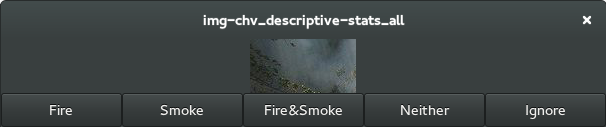
\includegraphics[width=\textwidth]{interview.png}
    \caption{La interfaz gráfica.}
\end{figure}

\subsection{Clases de regiones}
Se utilizan \textbf{5} clases (\refcode{\ExecAll}{exec/DescriptiveStatsAll.hs}):
\begin{enumerate}
    \item \verb|Fire|
    \item \verb|Smoke|
    \item \verb|Fire&Smoke|
    \item \verb|Neither|
    \item \verb|Ignore|
\end{enumerate}

Las instancias etiquetadas con \verb|Ignore| están a la espera de ser removidos.

\subsection{Formato ARFF}

Para la escritura de los datos se utiliza el proyecto \refcode{\WekaData}{WekaData}; el código fuente se incluye en la carpeta \verb|sources|.

Los adaptadores entre \verb|LearnDataEntry| y \verb|WekaEntry| se encuentran en\\ \refcode{\Weka}{src/ImgCharacteristics/Weka.hs}.

\subsection{Ejecutable}
El proyecto provee varios ejecutables, pero \verb|img-chv_descriptive-stats_all| es el que se usa (\refcode{\ExecAll}{exec/DescriptiveStatsAll.hs}).

Tiene dos modos de uso:
\begin{enumerate}
\item \texttt{img-chv\_descriptive-stats\_all} \textit{images relation target}
\item \texttt{img-chv\_descriptive-stats\_all} \verb|--dir| 
       \textit{directory relation target}
    \begin{itemize}[leftmargin=2cm]
        \item[\textit{images}]   --- enumeración de imágenes;
        \item[\textit{directory}]--- un directorio con imágenes a procesar;
        \item[\textit{relation}] --- nombre de la relación (\verb|@relation|);
        \item[\textit{target}]   --- el archivo \emph{*.arff} a escribir.
    \end{itemize}
\end{enumerate}

\subsection{Compilación}

Requiere:
\begin{itemize}
    \item The Glorious Glasgow Haskell Compilation System (GHC), version 7.10.3.
    \item Common Architecture for Building Applications and Libraries (CABAL),
          version $\geq$ 1.10.
    \item \emph{ghc-gtk3}, version $\geq$ 0.14 (puede ser complicada a compilar).
    \item Proyecto \emph{Nat}.
    \item Proyecto \emph{WekaData}.
\end{itemize}

Las demás dependencias deben ser resueltas por CABAL sin problemas.

\section{Experimentos en Weka}

Para automatizar el proceso de aprendizaje del perceptron, fue creado un pequeño proyecto en Scala \refcode{\WekaANN}{WekaANN}. Se aprovecha la facilidad de conexión de aplicaciones de JMV para correr las \emph{evaluaciones} de Weka.

\begin{itemize}
\item Prepara los datos, removiendo las instancias marcadas con la clase 
    \verb|Ignore|.
\item Guarda los reportes de Weka en archivos (por defecto en directorio ``reports'').
\end{itemize}

\medskip
En el directorio del proyecto \emph{scripts} se encuentran estos programas:
\begin{enumerate}
\item \verb|bulkANN.scala| --- fue utilizado para prueba de configuraciones diferentes.
\item \verb|findBestReports.scala| --- selecciona los mejores reportes (por el porcentaje de clasificación correcta).
\item \verb|extractReportsInfo.scala| --- extrae estadísticas desde los reportes y las escribe en un archivo.
\end{enumerate}

\medskip
En el directorio \verb|octave| se encuentran diferentes utilidades para graficar los comparaciones de los resultados (para Matlab/Octave).

\subsection{Configuraciones de la red}

Fueron realizados experimentos con todas las combinaciones de los siguientes valores:

\begin{center}
\begin{tabular}{l}
\begin{tabular}{|l|l|}
\hline
Variable 					& Valores				\\
\hline
Número de épocas			& 500, 1000, 2000, 3000 \\
``Learning rate''  	    	& 0.1, 0.2, 0.5, 0.8 	\\
``Momentum''				& 0.2, 0.5, 0.8 		\\
$1^{\text{ra}}$ capa oculta	& a, t					\\
$2^{\text{da}}$ capa oculta	& 0, a, t				\\
\hline
\end{tabular}\\
\textbf{Total:} 288 combinaciones.
\end{tabular}
\end{center}

\def\valT{61}
\def\valA{30}

$t=\text{núm. de classes} + \text{núm. de attributos} = 56+5=\valT; a=\dfrac{t}{2}=\valA$.

%Inicialmente se planeaba hacer pruebas con las combinaciones de las siguientes configuraciones:


\section{Análisis de resultados}

\begin{table}
\begin{tabular}{|l||l|l|l|l|l||l|l|}
\hline
\# & épocas & learn. & mom. & capa 1 & capa 2 & clasificado & rel. abs. err. \\
\hline
 1& 500    & 0.1    & 0.5    & t    & a    & 78.3044 \%  & 32.4691 \% \\
 2& 500    & 0.1    & 0.5    & t    & t    & 78.1464 \%  & 32.8638 \% \\
 3& 3000   & 0.1    & 0.2    & t    & a    & 78.0411 \%  & 32.1325 \% \\
 4& 3000   & 0.1    & 0.2    & t    &      & 77.8831 \%  & 34.6127 \% \\
 5& 1000   & 0.1    & 0.8    & t    & t    & 77.8304 \%  & 33.1316 \% \\
 6& 1000   & 0.1    & 0.2    & t    & a    & 77.7251 \%  & 33.4992 \% \\
 7& 1000   & 0.1    & 0.2    & t    &      & 77.7251 \%  & 35.4322 \% \\
 8& 3000   & 0.1    & 0.5    & t    &      & 77.6198 \%  & 34.8487 \% \\
 9& 1000   & 0.2    & 0.8    & t    & t    & 77.6198 \%  & 33.7434 \% \\
10& 2000   & 0.5    & 0.2    & t    & t    & 77.6198 \%  & 33.8068 \% \\
\hline
\end{tabular}
\caption{Las configuraciones con los mejores resultados.}
\label{table:results_best}
\end{table}

\begin{table}
\begin{tabular}{|l||l|l|l|l|l||l|l|}
\hline
\# & épocas & learn. & mom. & capa 1 & capa 2 & clasificado & rel. abs. err. \\
\hline
 1& 3000   & 0.8    & 0.8    & a    & t    & 11.743  \%   & 125.7089 \% \\
 2& 2000   & 0.8    & 0.8    & t    & t    & 15.3765 \%   & 120.8736 \% \\
 3& 1000   & 0.8    & 0.8    & t    & t    & 16.7983 \%   & 120.174  \% \\
 4& 3000   & 0.8    & 0.8    & t    & t    & 20.5898 \%   & 115.5593 \% \\
 5& 2000   & 0.8    & 0.8    & a    & t    & 22.9595 \%   & 111.3145 \% \\
\hline
\end{tabular}
\caption{Las configuraciones con los peores resultados.}
\label{table:results_worst}
\end{table}

Para analizar la influencia de diferentes variables sobre la calidad de aprendizaje,
fueron graficados unas proyecciones, los cuales parecen a una histograma, de siguiente manera:

\begin{flalign*}
\text{Sean } &C={c_i} \text{ --- variables configurables.}\\
			 &E={e_i} \text{ --- estadísticas para las configuraciones.}\\
			 &D={d_j} \text{ --- arreglos de configuraciones, tales que}\\
			 &\qquad\begin{aligned}
			 	\forall d_j &\in D  \\
			 	& \forall c_i \in C ~ \exists \text{ un valor } d^c_{ij}
			 		\text{ asociado -- el valor de la variable } c_i\\
			 	&	\qquad \text{ en la configuración } d_j;\\
			 	&\forall e_i \in E ~ \exists \text{ un valor } d^e_{ij}
			 		\text{ asociado -- el valor de la estadística } e_i\\
			 	&	\qquad \text{ en la configuración } d_j.
			 \end{aligned}\\
\end{flalign*}
Una proyección de variables $X,Y \in C$ sobre la estadística $Z \in E$ con operador $op$ es
el conjunto de valores $\{p_{xy}\}$, tales que
\begin{flalign*}
& \forall \text{ único } x \in \text{ valores de } X \\
& \forall \text{ único } y \in \text{ valores de } Y \\
& p_{xy} = op(\{z_{xy}\}) \text{, donde} \\
& \{z_{xy}\} = \left\lbrace d^e_{Zj} ~|~ \forall d_j \in D
	\textbf{ si } d^c_{Xk} = x \wedge d^Y_{Yk} = y \right\rbrace\\		
\end{flalign*}

El operador $op$ puede ser el \emph{promedio}, o valor \emph{máximo/mínimo}, 
u otra función con tipo $\{z\} \mapsto z$.


\begin{figure}[h]
	\centering
	\begin{subfigure}[b]{0.49\textwidth}
        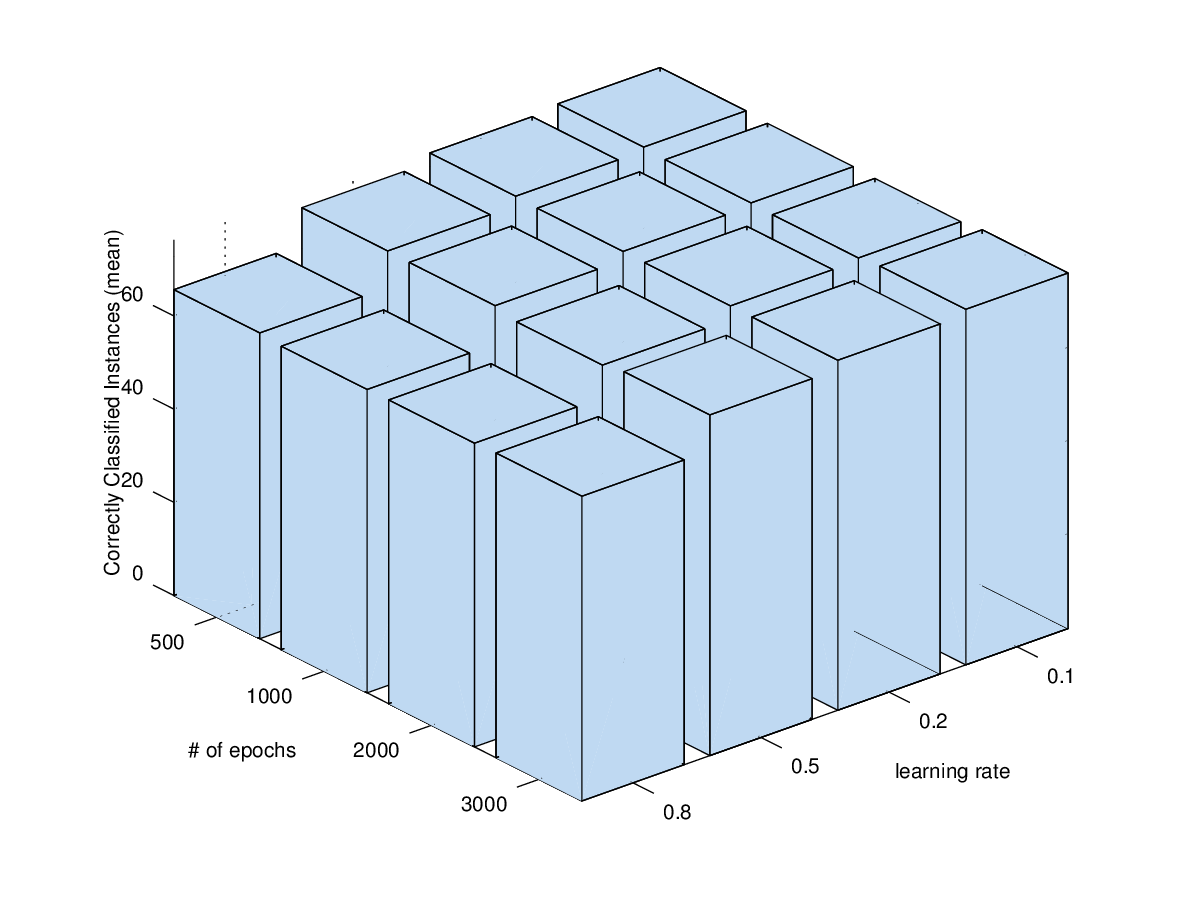
\includegraphics[width=\textwidth]{plots/cmean_NL.png}
        \caption{Escala lineal.}
        \label{fig:cmean_NL-lin}
    \end{subfigure}
	\begin{subfigure}[b]{0.49\textwidth}
        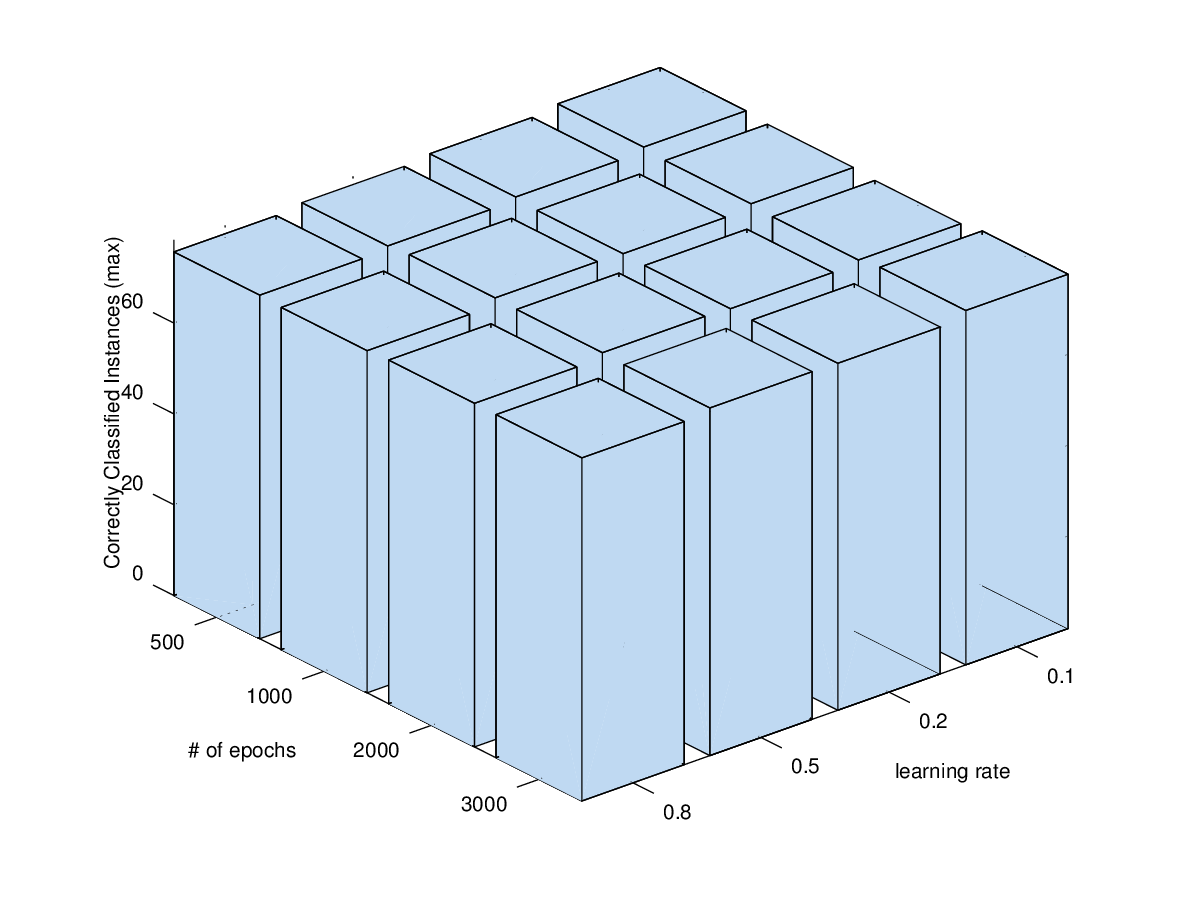
\includegraphics[width=\textwidth]{plots/cmax_NL.png}
        \caption{Escala lineal.}
        \label{fig:cmax_NL-lin}
    \end{subfigure}
    \\
	\begin{subfigure}[b]{0.49\textwidth}
        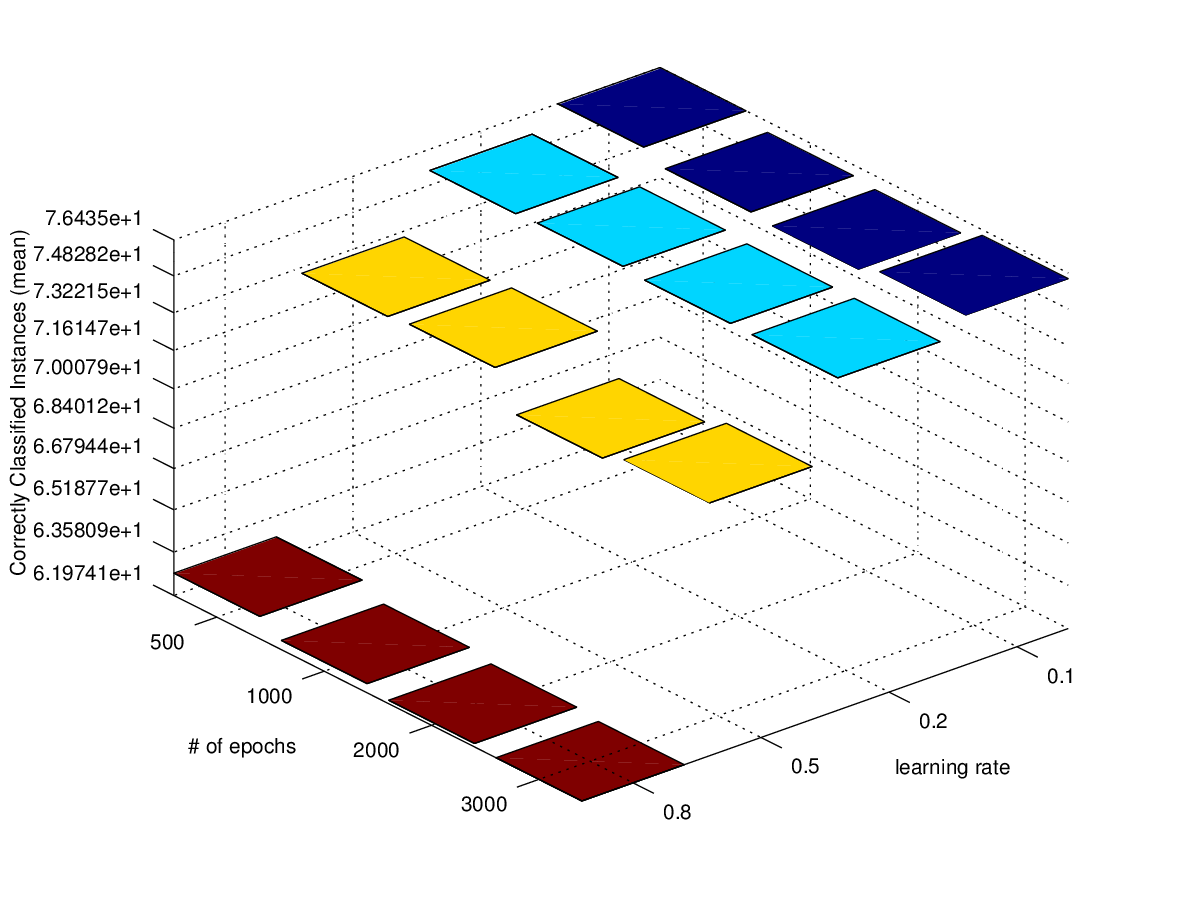
\includegraphics[width=\textwidth]{plots/cmean_NL-log.png}
        \caption{Escala logarítmica.}
        \label{fig:cmean_NL-log}
    \end{subfigure}
	\begin{subfigure}[b]{0.49\textwidth}
        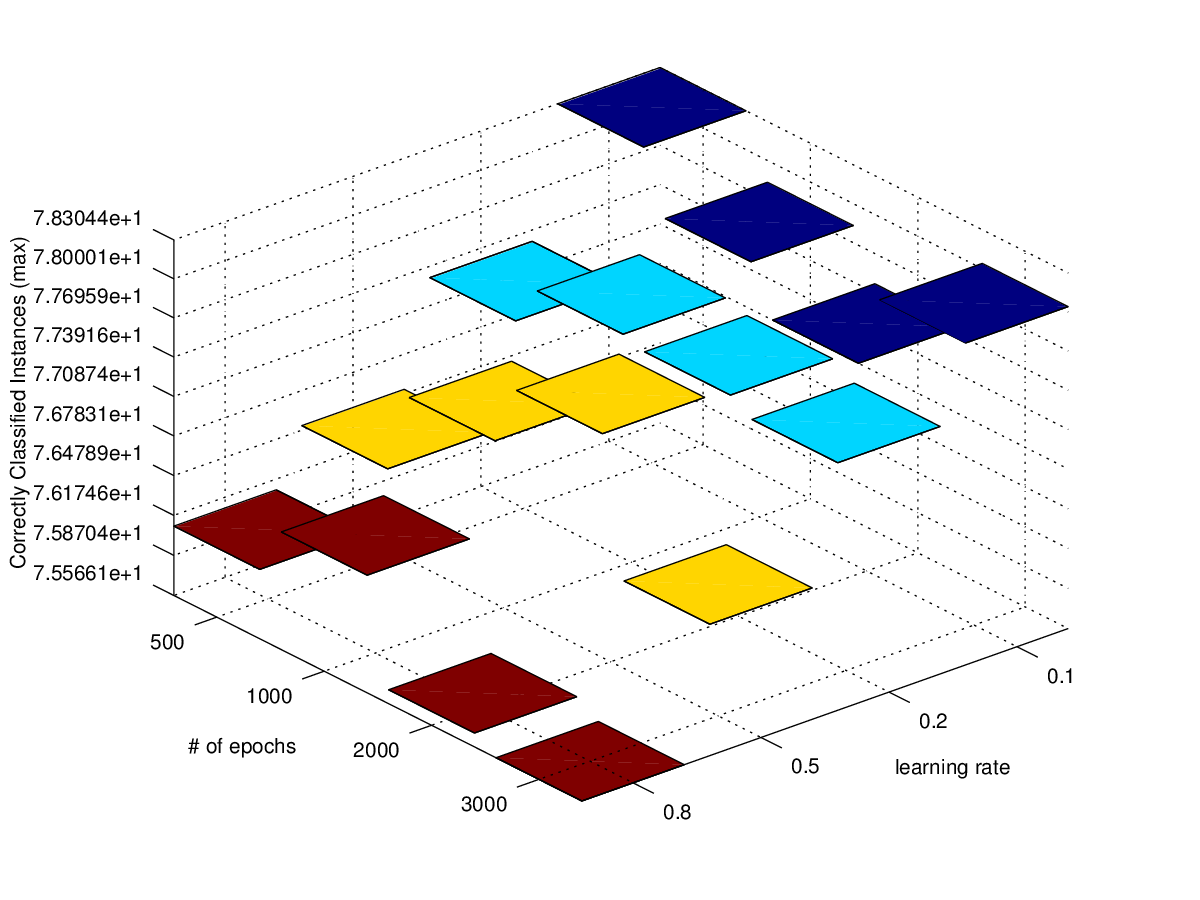
\includegraphics[width=\textwidth]{plots/cmax_NL-log.png}
        \caption{Escala logarítmica.}
        \label{fig:cmax_NL-log}
    \end{subfigure}    
	
	\caption{La proyección del \emph{número de épocas} utilizado y el \emph{``learning rate''} 
			 sobre la \textbf{media} (izquierda: \ref{fig:cmean_NL-lin}, \ref{fig:cmean_NL-log})
			 y el \textbf{máximo} (derecha: \ref{fig:cmax_NL-lin}, \ref{fig:cmax_NL-log})
			 del \emph{número de instancias correctamente clasificadas}. 
			}
	\label{fig:NL}
\end{figure}


\begin{figure}[h]
	\centering
	\begin{subfigure}[b]{0.49\textwidth}
        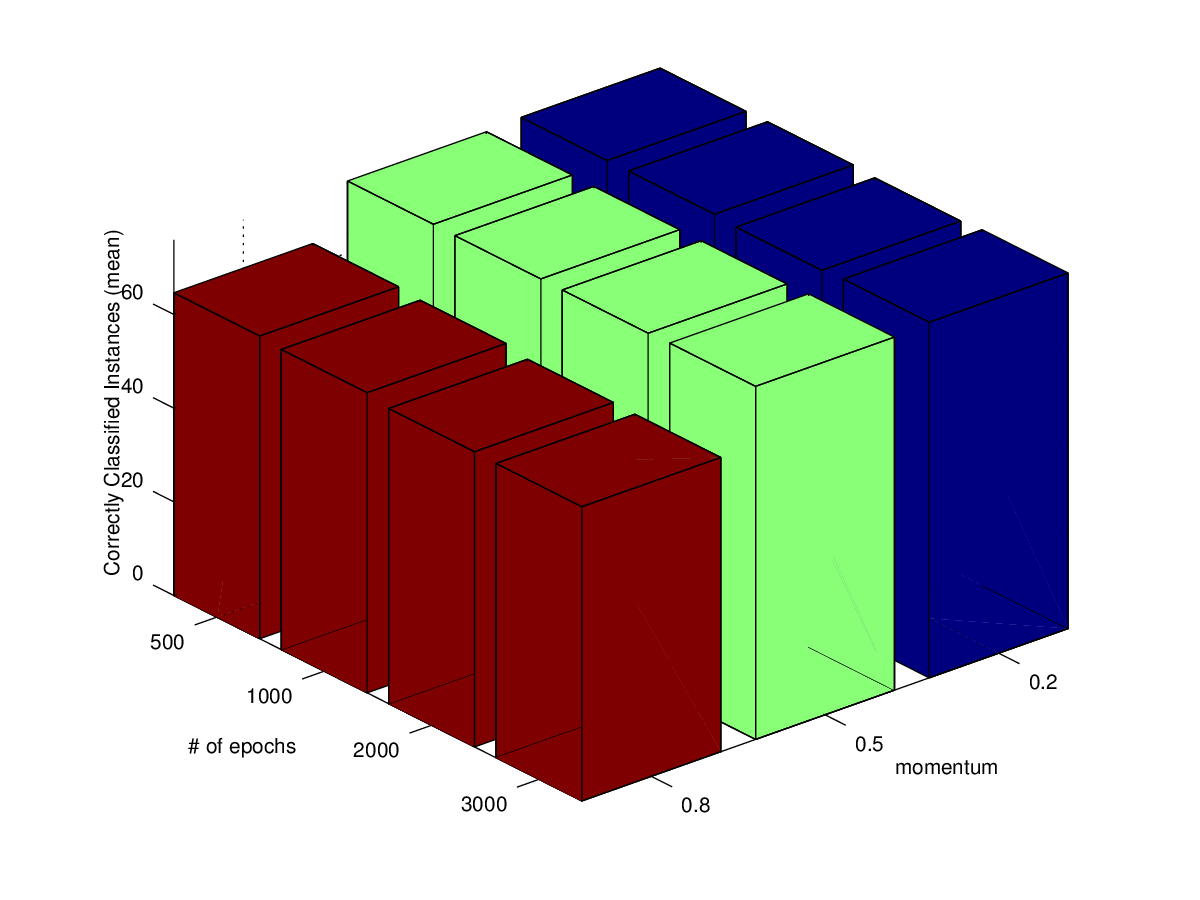
\includegraphics[width=\textwidth]{plots/cmean_NM.png}
        \caption{Escala lineal.}
        \label{fig:cmean_NM-lin}
    \end{subfigure}
	\begin{subfigure}[b]{0.49\textwidth}
        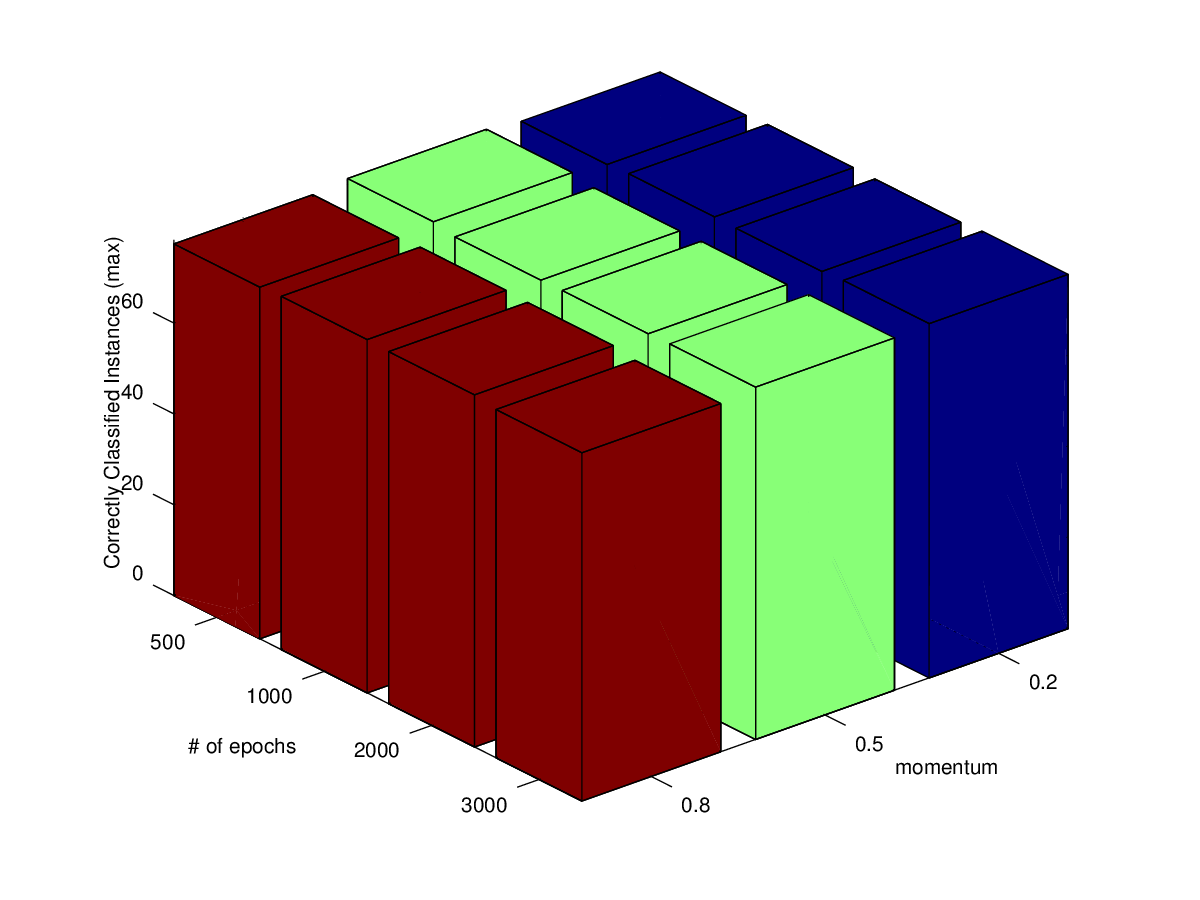
\includegraphics[width=\textwidth]{plots/cmax_NM.png}
        \caption{Escala lineal.}
        \label{fig:cmax_NM-lin}
    \end{subfigure}
    \\
	\begin{subfigure}[b]{0.49\textwidth}
        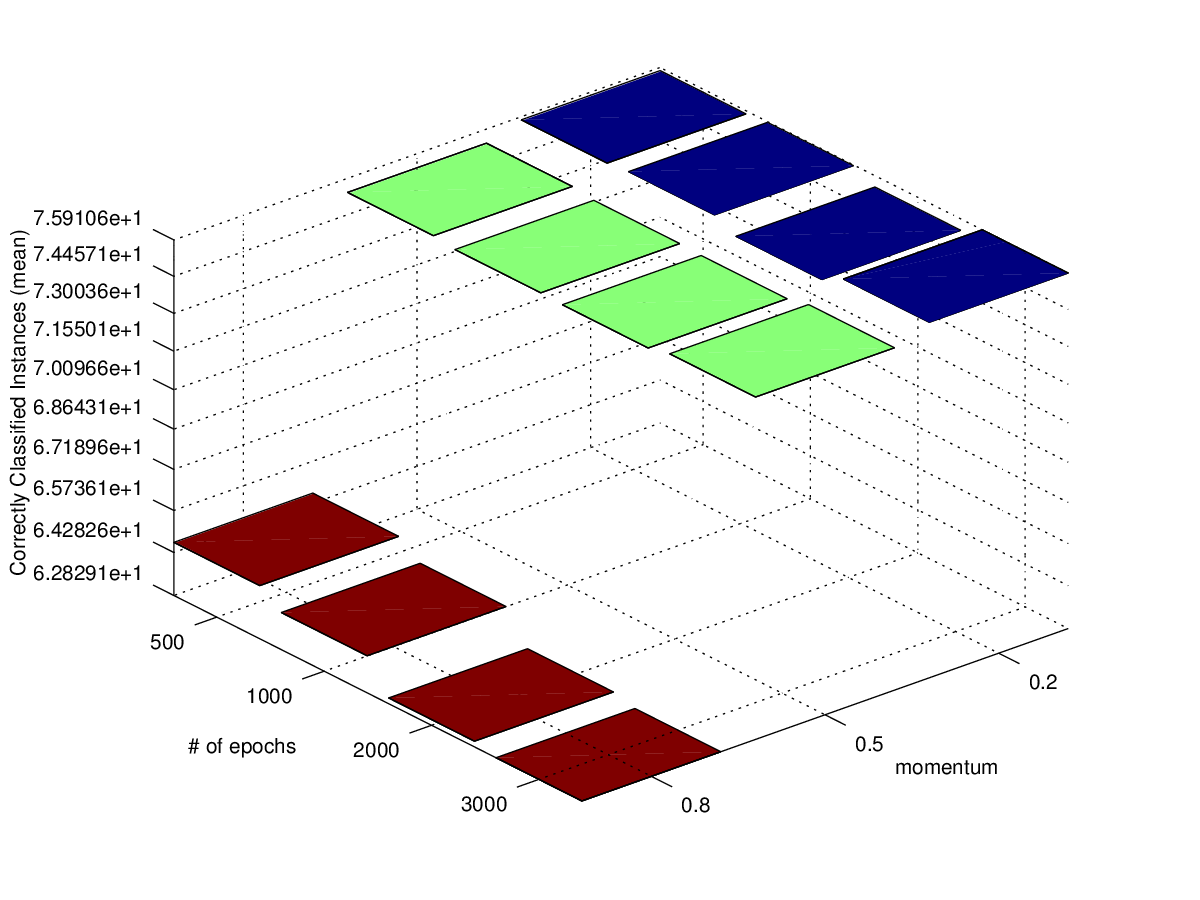
\includegraphics[width=\textwidth]{plots/cmean_NM-log.png}
        \caption{Escala logarítmica.}
        \label{fig:cmean_NM-log}
    \end{subfigure}
	\begin{subfigure}[b]{0.49\textwidth}
        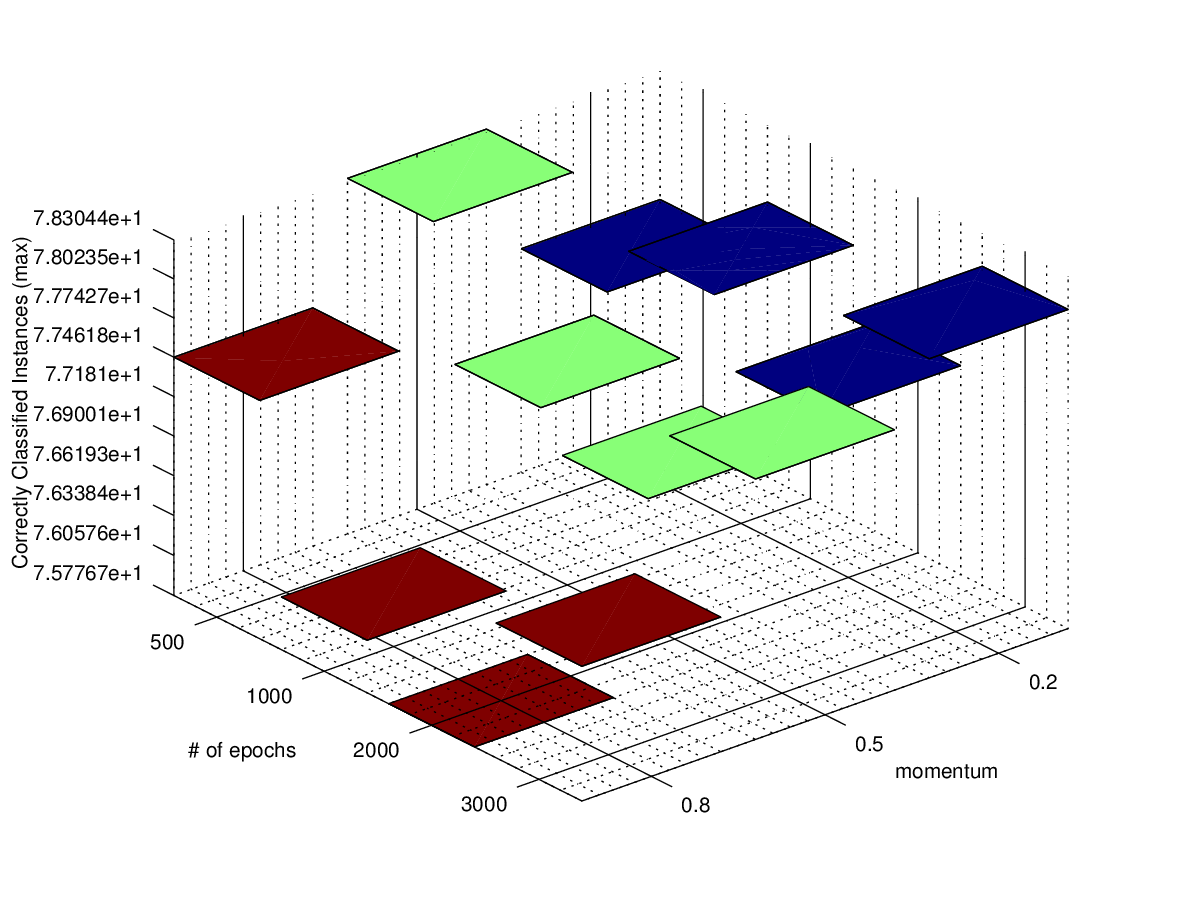
\includegraphics[width=\textwidth]{plots/cmax_NM-log.png}
        \caption{Escala logarítmica.}
        \label{fig:cmax_NM-log}
    \end{subfigure}    
	
	\caption{La proyección del \emph{número de épocas} utilizado y el \emph{``momentum''} 
			 sobre la \textbf{media} 
			 (izquierda: \ref{fig:cmean_NM-lin}, \ref{fig:cmean_NM-log}) 
			 y el \textbf{máximo} (derecha: \ref{fig:cmax_NM-lin}, \ref{fig:cmax_NM-log})
			 del \emph{número de instancias correctamente clasificadas}. }
	\label{fig:NM}
\end{figure}

\begin{figure}[h]
	\centering
	\begin{subfigure}[b]{0.49\textwidth}
        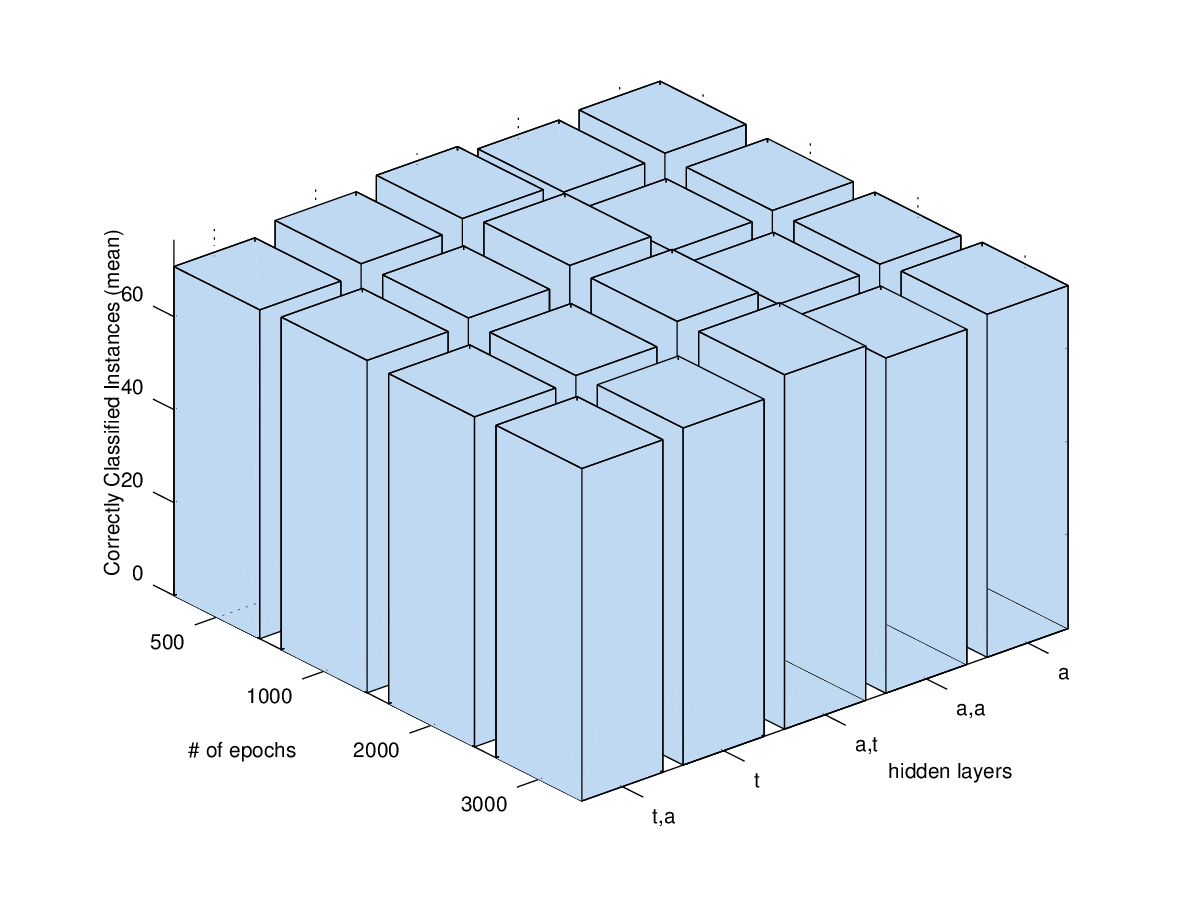
\includegraphics[width=\textwidth]{plots/cmean_NH.png}
        \caption{Escala lineal.}
        \label{fig:cmean_NH-lin}
    \end{subfigure}
	\begin{subfigure}[b]{0.49\textwidth}
        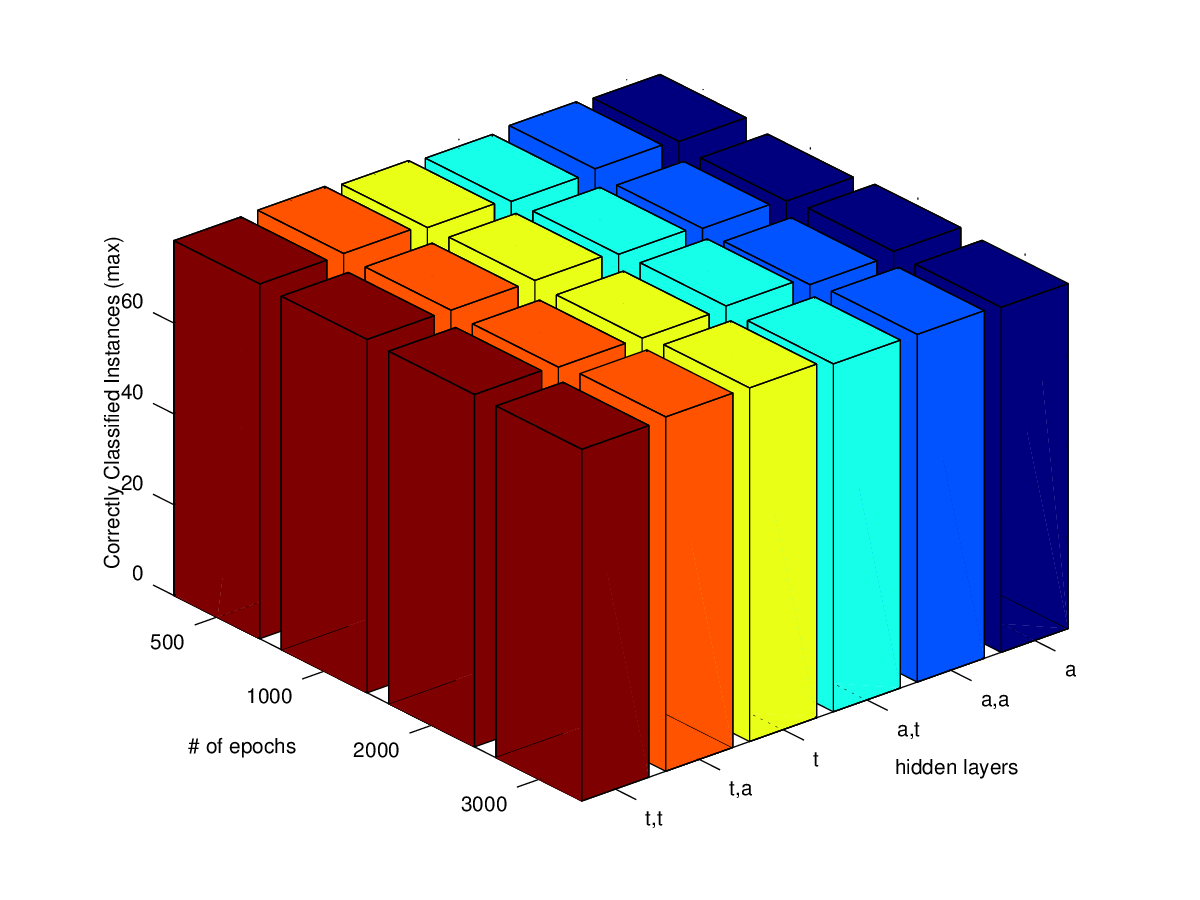
\includegraphics[width=\textwidth]{plots/cmax_NH.png}
        \caption{Escala lineal.}
        \label{fig:cmax_NH-lin}
    \end{subfigure}
    \\
	\begin{subfigure}[b]{0.49\textwidth}
        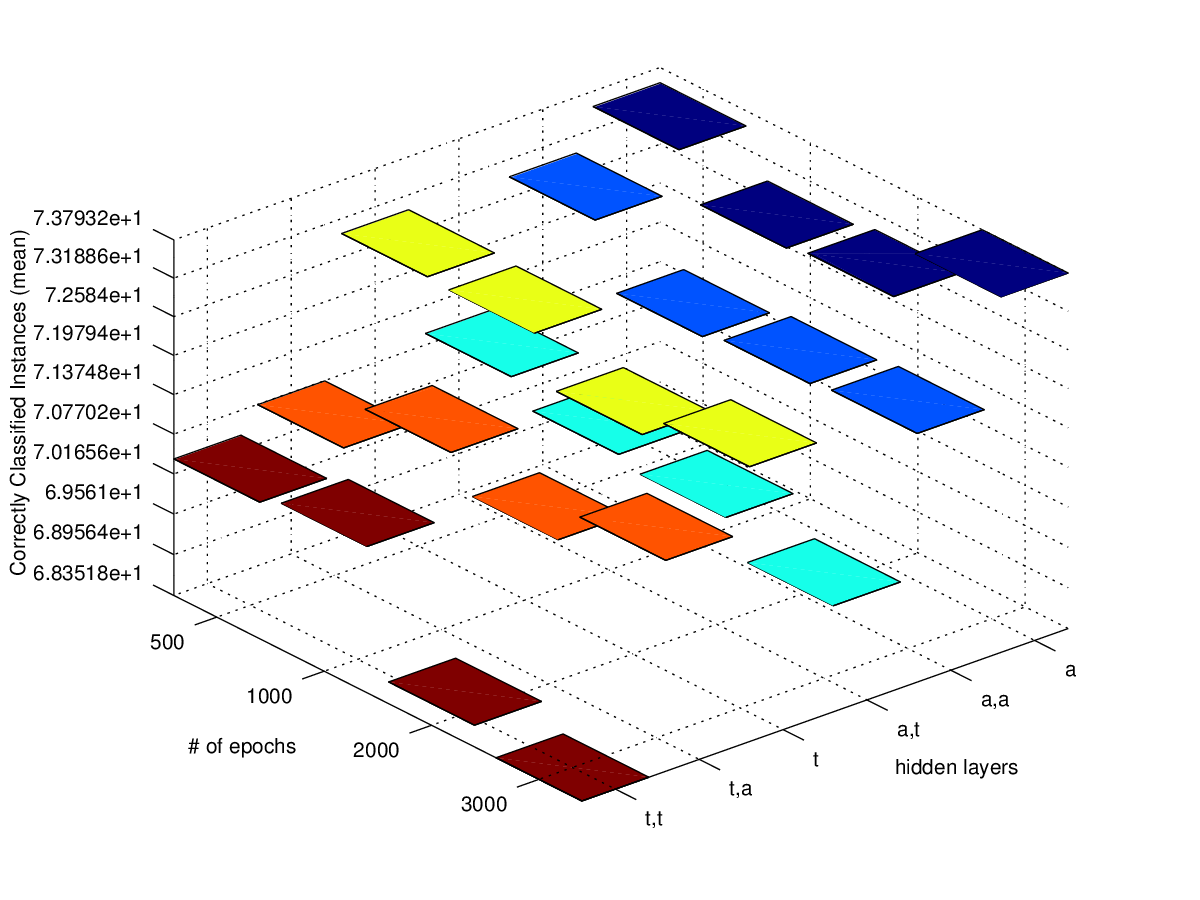
\includegraphics[width=\textwidth]{plots/cmean_NH-log.png}
        \caption{Escala logarítmica.}
        \label{fig:cmean_NH-log}
    \end{subfigure}
	\begin{subfigure}[b]{0.49\textwidth}
        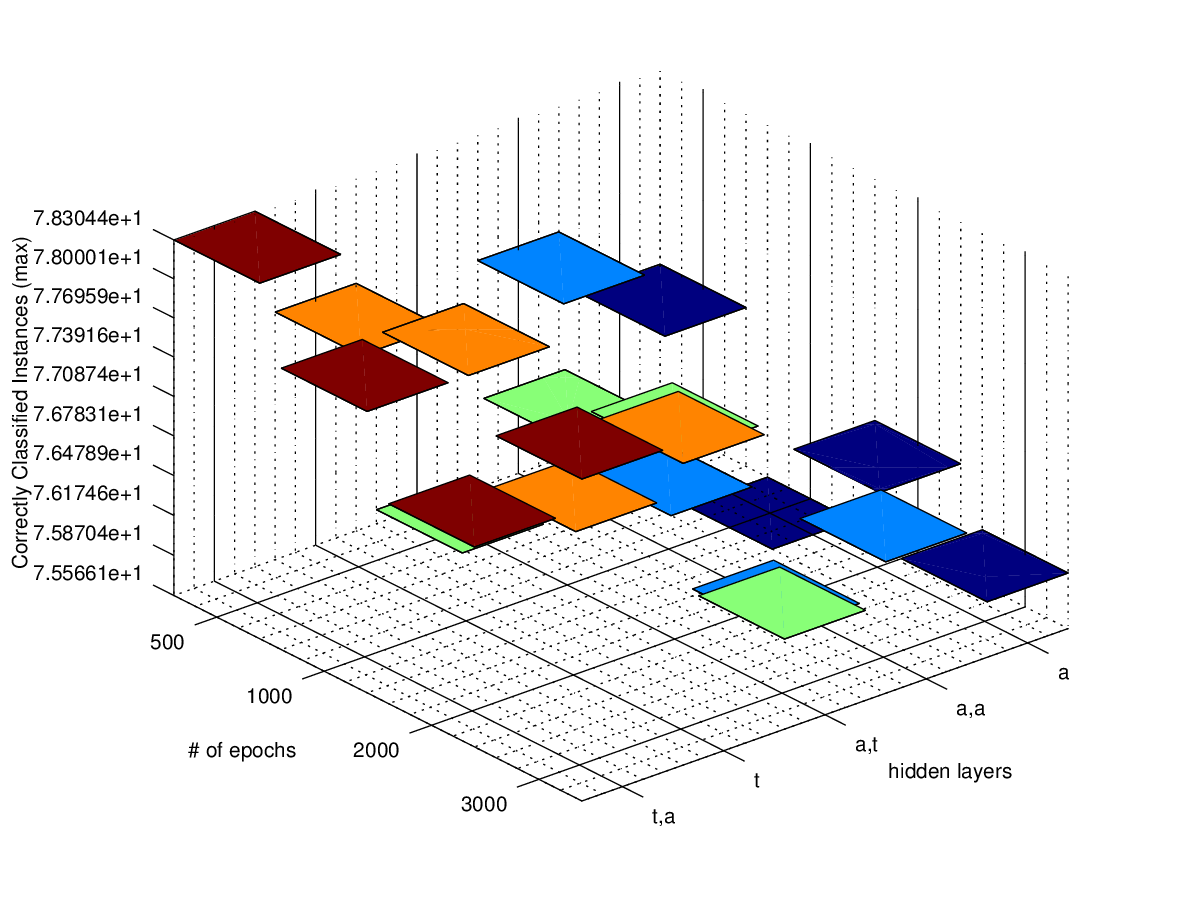
\includegraphics[width=\textwidth]{plots/cmax_NH-log.png}
        \caption{Escala logarítmica.}
        \label{fig:cmax_NH-log}
    \end{subfigure}    
	
	\caption{La proyección del \emph{número de épocas} utilizado y la
			 \emph{configuración de las capas escondidas} 
			 sobre la \textbf{media} (izquierda: \ref{fig:cmean_NH-lin}, \ref{fig:cmean_NH-log})
			 y el \textbf{máximo} (derecha: \ref{fig:cmax_NH-lin}, \ref{fig:cmax_NH-log})
			 del \emph{número de instancias correctamente clasificadas}.}
	\label{fig:NHc}
\end{figure}

\begin{figure}[h]
	\centering
	\begin{subfigure}[b]{0.49\textwidth}
        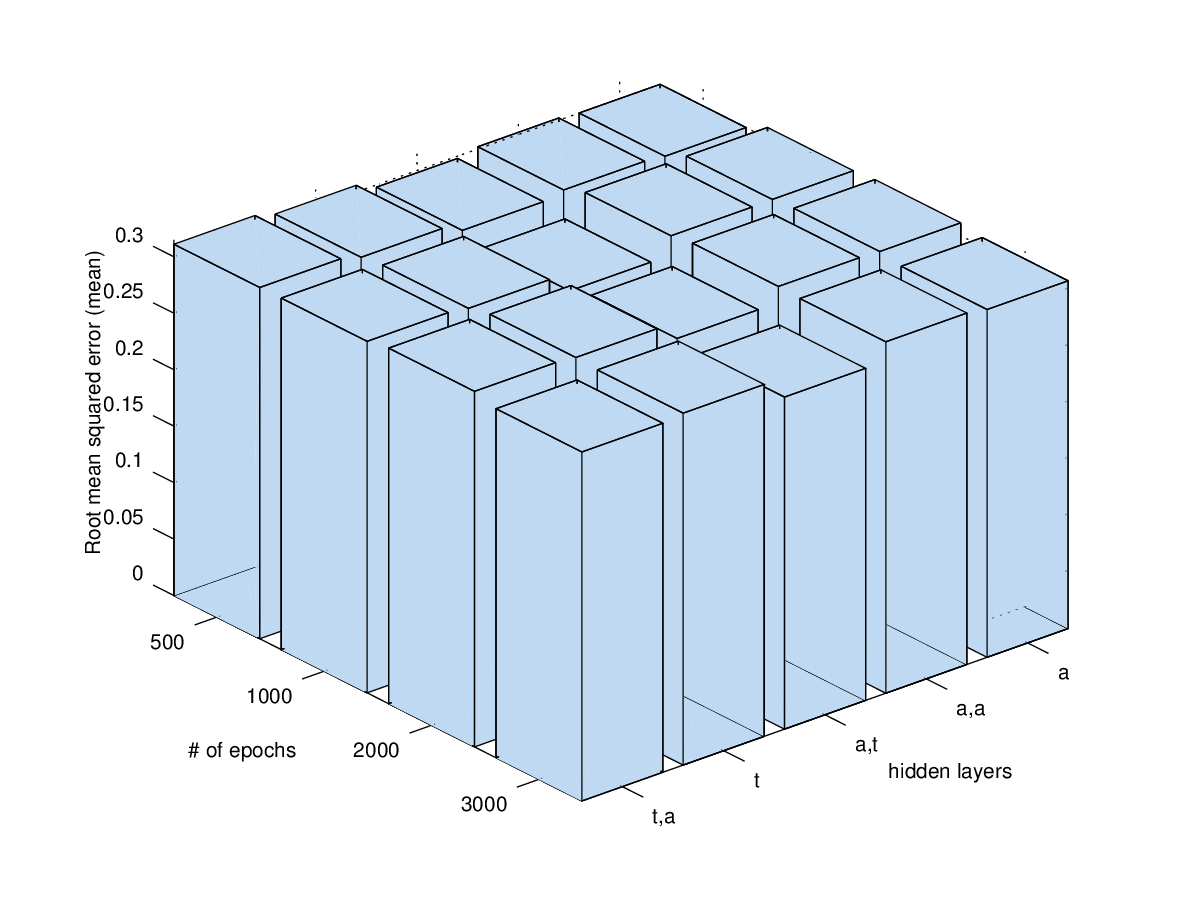
\includegraphics[width=\textwidth]{plots/emean_NH.png}
        \caption{Escala lineal.}
        \label{fig:emean_NH-lin}
    \end{subfigure}
	\begin{subfigure}[b]{0.49\textwidth}
        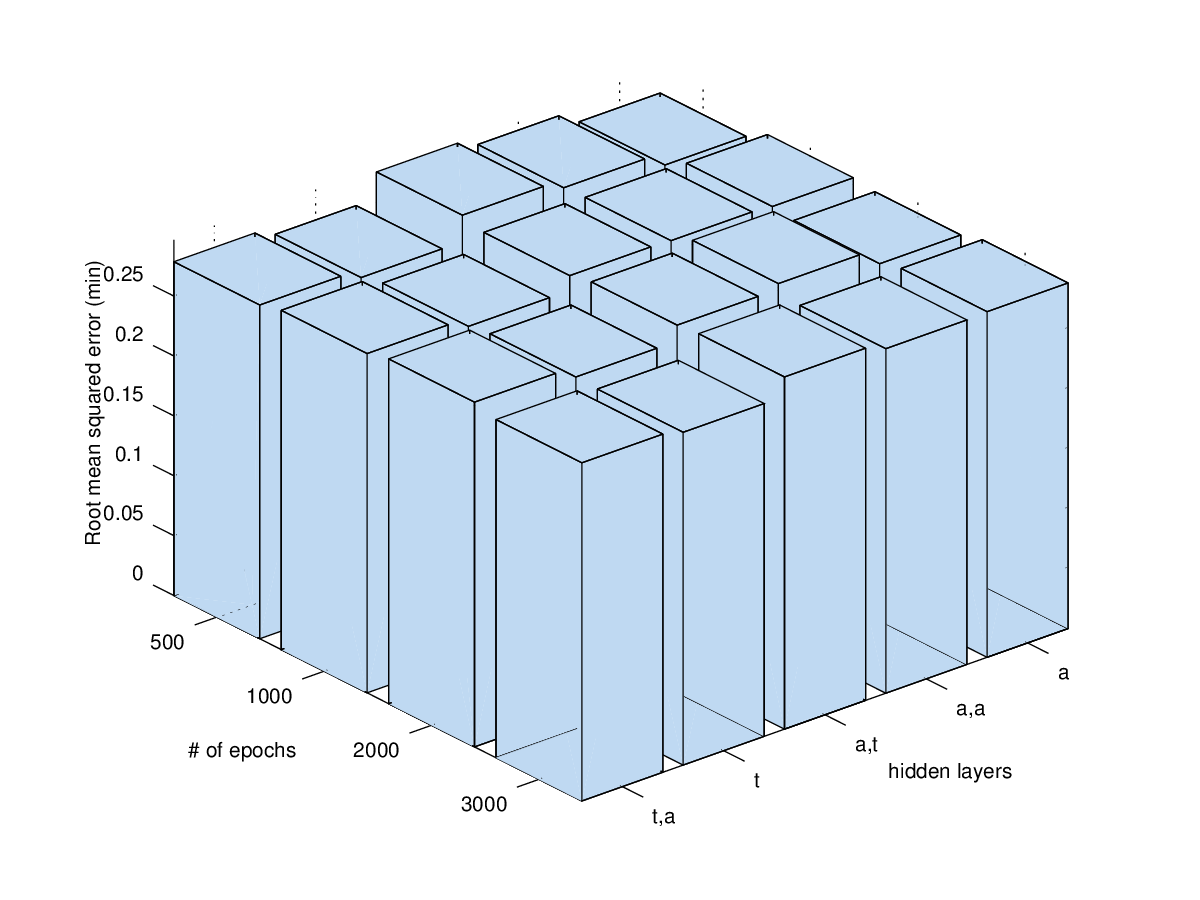
\includegraphics[width=\textwidth]{plots/emin_NH.png}
        \caption{Escala lineal.}
        \label{fig:emin_NH-lin}
    \end{subfigure}
    \\
	\begin{subfigure}[b]{0.49\textwidth}
        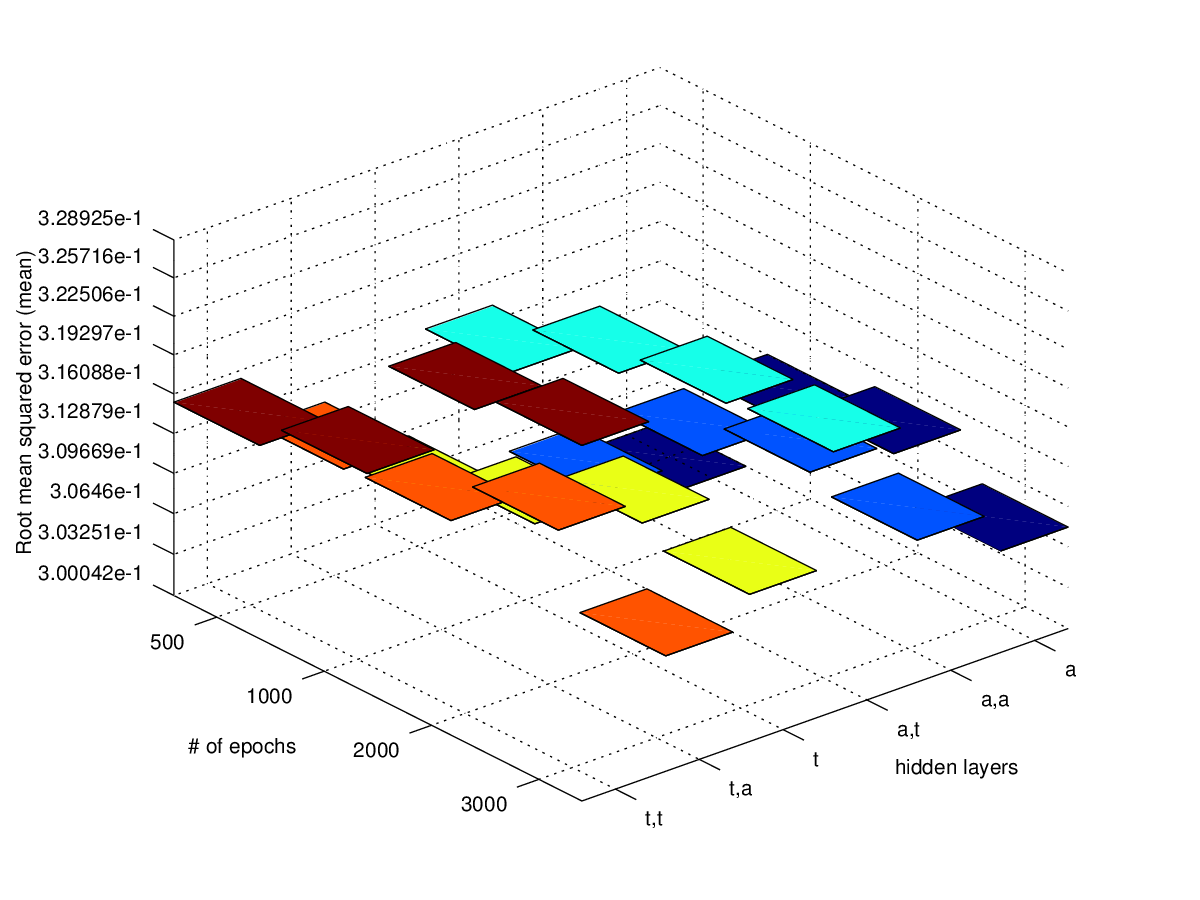
\includegraphics[width=\textwidth]{plots/emean_NH-log.png}
        \caption{Escala logarítmica.}
        \label{fig:emean_NH-log}
    \end{subfigure}
	\begin{subfigure}[b]{0.49\textwidth}
        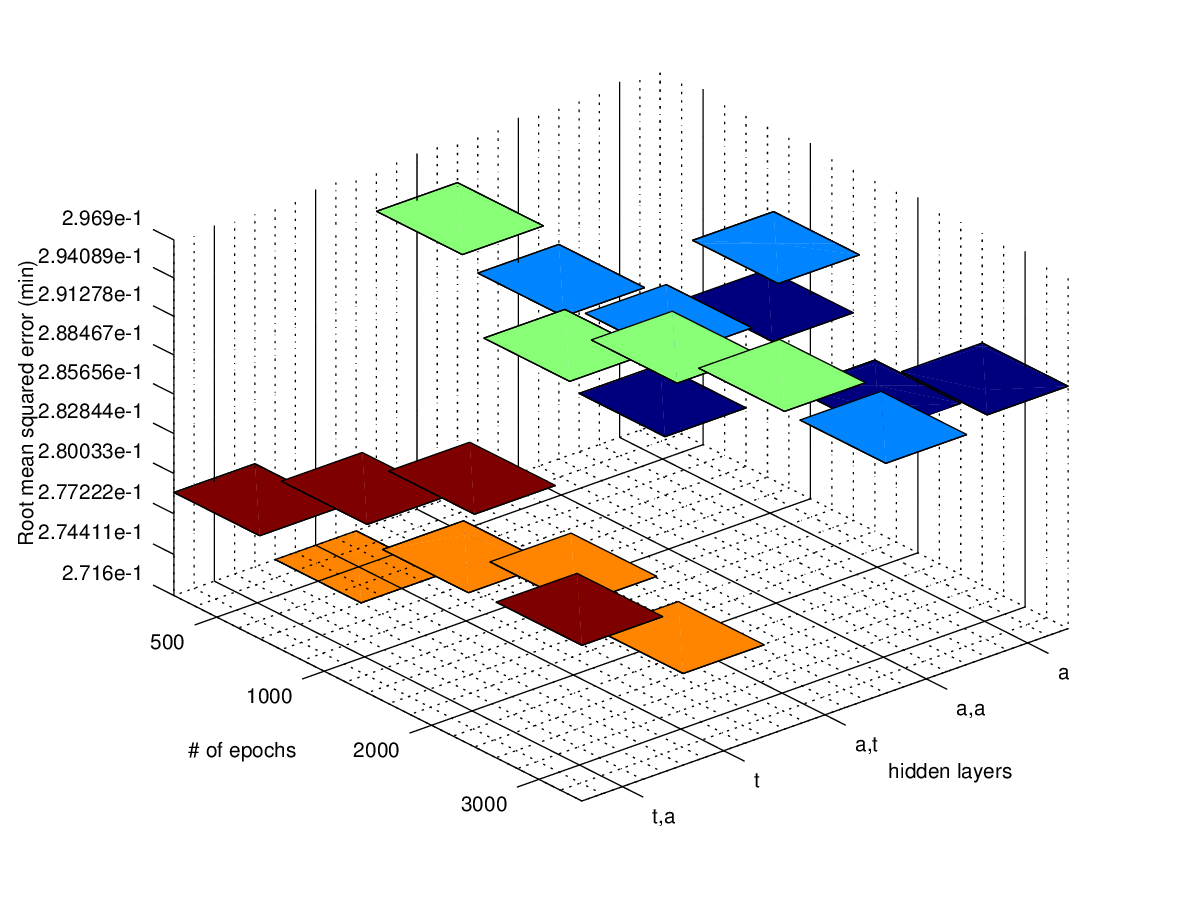
\includegraphics[width=\textwidth]{plots/emin_NH-log.png}
        \caption{Escala logarítmica.}
        \label{fig:emin_NH-log}
    \end{subfigure}    
	
	\caption{La proyección del \emph{número de épocas} utilizado y la
			 \emph{configuración de las capas escondidas} 
			 sobre la \textbf{media} (izquierda: \ref{fig:emean_NH-lin}, \ref{fig:emean_NH-log}) 
			 y el \textbf{mínimo} (derecha: \ref{fig:emin_NH-lin}, \ref{fig:emin_NH-log})
			 de la \emph{error cuadrática media}.}
	\label{fig:NHe}
\end{figure}
	


%\begin{figure}[h]
%	\centering
%	\begin{subfigure}[b]{0.49\textwidth}
%        \includegraphics[width=\textwidth]{plots/.png}
%        \caption{Escala lineal.}
%        \label{fig:-lin}
%    \end{subfigure}
%	\begin{subfigure}[b]{0.49\textwidth}
%        \includegraphics[width=\textwidth]{plots/.png}
%        \caption{Escala lineal.}
%        \label{fig:-lin}
%    \end{subfigure}
%    \\
%	\begin{subfigure}[b]{0.49\textwidth}
%        \includegraphics[width=\textwidth]{plots/-log.png}
%        \caption{Escala logarítmica.}
%        \label{fig:-log}
%    \end{subfigure}
%	\begin{subfigure}[b]{0.49\textwidth}
%        \includegraphics[width=\textwidth]{plots/-log.png}
%        \caption{Escala logarítmica.}
%        \label{fig:-log}
%    \end{subfigure}    
%	
%	\caption{}
%	\label{fig:}
%\end{figure}

% % % % % % % % % % % % % % % % % % % % % % % % % % % % % % % % % % % % % % % % % % % % %

Se puede ver que los gráficos en la figura \ref{fig:NHe} son una reflexión de los gráficos en la figura \ref{fig:NHc}.

Pueden hacerse las siguientes conclusiones:

\subsection{Influencia de ``learning rate''}
La calidad disminuye con el aumento del ``learning rate'' (figura \ref{fig:NL}). 
Las 5 configuraciones, que mostraron los peores resultados (tabla \ref{table:results_worst}), todos tenían el l.r. máximo de las pruebas (0.8).

\subsection{Influencia de ``momentum''}
En la figura \ref{fig:NM} se puede ver que el mayor valor (0.8) del ``momentum''         
produjo los peores resultados. La diferencia de los promedios para $0.5$ y $0.2$ está 
ligeramente en favor del valor menor, mientras que los máximos son inconclusos.

\subsection{Influencia de la capa oculta}
\begin{enumerate}[a).]
\item Las 10 mejores configuraciones tenían $t=\dfrac{a}{2} = \valT$ neuronas en la primera 
      capa. En las figuras \ref{fig:NHc}, \ref{fig:NHe} y tabla \ref{table:results_best} se 
      puede ver que
      \begin{itemize}
          \item los mejores resultados (los máximos) fueron producidos por las redes de dos 
                capas: $t,a = \valT,\valA$ y $t,t = \valT,\valT$.
          \item la configuración con el resultado siguiente fue de una sola capa $t=\valT$.
          \item los peores máximos fueron dados por la configuración $a=\valA$.
      \end{itemize}
\item Pero en las figuras \ref{fig:NHc} y \ref{fig:NHe} se puede ver que en promedio, 
      los mejores resultados fueron dados por la configuración de una capa: $a=\valA$. Esto significa que está menos influenciada por los 
      demás parámetros.
      Igual, las redes $t,a$ y $t,t$ mostraron promedios notablemente peores que sus 
      máximos.
\item La configuración $a,t=\valA,\valT$ no mostró ni bien máximo, ni bien promedio.
\end{enumerate}

\subsection{Matrices de confusión}

\begin{enumerate}
\item \verb|Fire&Smoke| mostró el peor ratio de clasificación \emph{verdadera positiva}.
\item \verb|Neither| mostró el mejor ratio de clasificación \emph{verdadera positiva}, 
                     después sigue \verb|Smoke|.
\item \verb|Neither| también demuestra el mayor ratio de clasificación
                     \emph{falsa positiva}.
\item El menor ratio de clasificación \emph{falsa positiva} fue mostrado por clases
      \verb|Fire| y \verb|Fire&Smoke|.
\item Aun que la clase \verb|Neither| mostró el peor ratio de falsas positivas, 
      demuestra también la mejor precisión entre las clases.
\item \verb|Fire&Smoke| tiene la peor precisión de las clases utilizadas.
\end{enumerate}

Cómo se puede puede ver en la figura \ref{fig:classes}:
\begin{itemize}
\item Las clases \verb|Fire| y \verb|Smoke| se distinguen bien.
\item Se distingue bien \verb|Neither| de \verb|Fire|, pero no al contrario.
\item La clase \verb|Fire&Smoke| se distingue mal de ambos \verb|Fire| y \verb|Smoke|.
\item \verb|Fire| se distingue mal de \verb|Fire&Smoke|.
\item \verb|Fire| y \verb|Smoke| tienen en porcentaje de equivocaciones en favor de 
      \verb|Neither| parecido ($\approx 14\%$).
\end{itemize}

% % % % % % % % % % % % % % % % % % % % % % % % % % % % % % % % % % % % % % % % % % % % %
\begin{figure}[h]
    \centering
    \footnotesize
    \renewcommand{\thesubfigure}{\arabic{subfigure}}
 
    \begin{subfigure}[b]{\textwidth}
    \caption{}
    \label{fig:cmatrix01}
    \begin{lstlisting}[language={}, basicstyle=\footnotesize, frame=none, basewidth=0.45em]
			   a   b   c   d   e   <-- classified as
			 200   8  49  41   0 |   a = Fire
			  12 407  29  70   0 |   b = Smoke
			  54  41 132  22   0 |   c = Fire&Smoke
			  28  51   7 748   0 |   d = Neither
			   0   0   0   0   0 |   e = Ignore

               TP Rate   FP Rate   Precision   Recall  F-Measure   ROC Area  Class
                 0.671     0.059      0.68      0.671     0.676      0.901    Fire
                 0.786     0.072      0.803     0.786     0.794      0.928    Smoke
                 0.53      0.052      0.608     0.53      0.567      0.869    Fire&Smoke
                 0.897     0.125      0.849     0.897     0.872      0.931    Neither
                 0         0          0         0         0          ?        Ignore
Weighted Avg.    0.783     0.091      0.778     0.783     0.78       0.917
    \end{lstlisting} 
    \end{subfigure}


    \begin{subfigure}[b]{\textwidth}
    \caption{}
    \label{fig:cmatrix02}
    \begin{lstlisting}[language={}, basicstyle=\footnotesize, frame=none, basewidth=0.45em]
			   a   b   c   d   e   <-- classified as
			 212   7  46  33   0 |   a = Fire
			   6 413  35  64   0 |   b = Smoke
			  62  50 121  16   0 |   c = Fire&Smoke
			  38  33  25 738   0 |   d = Neither
			   0   0   0   0   0 |   e = Ignore

               TP Rate   FP Rate   Precision   Recall  F-Measure   ROC Area  Class
                 0.711     0.066      0.667     0.711     0.688      0.919    Fire
                 0.797     0.065      0.821     0.797     0.809      0.921    Smoke
                 0.486     0.064      0.533     0.486     0.508      0.865    Fire&Smoke
                 0.885     0.106      0.867     0.885     0.876      0.945    Neither
                 0         0          0         0         0          ?        Ignore
Weighted Avg.    0.781     0.083      0.779     0.781     0.78       0.924
    \end{lstlisting}
    \end{subfigure} 
    
    
    \begin{subfigure}[b]{\textwidth}
    \caption{}
    \label{fig:cmatrix03}
    \begin{lstlisting}[language={}, basicstyle=\footnotesize, frame=none, basewidth=0.45em]
			   a   b   c   d   e   <-- classified as
			 201  13  41  43   0 |   a = Fire
			   7 417  46  48   0 |   b = Smoke
			  54  48 130  17   0 |   c = Fire&Smoke
			  31  49  20 734   0 |   d = Neither
			   0   0   0   0   0 |   e = Ignore

               TP Rate   FP Rate   Precision   Recall  F-Measure   ROC Area  Class
                 0.674     0.057      0.686     0.674     0.68       0.91     Fire
                 0.805     0.08       0.791     0.805     0.798      0.93     Smoke
                 0.522     0.065      0.549     0.522     0.535      0.87     Fire&Smoke
                 0.88      0.101      0.872     0.88      0.876      0.938    Neither
                 0         0          0         0         0          ?        Ignore
Weighted Avg.    0.78      0.084      0.778     0.78      0.779      0.922
    \end{lstlisting}
    \end{subfigure}
\phantomcaption
\end{figure}


\clearpage
\begin{figure}[h]
\ContinuedFloat 
\renewcommand{\thesubfigure}{\arabic{subfigure}}

    \begin{subfigure}[b]{\textwidth}
    \caption{}
    \label{fig:cmatrix04}
    \begin{lstlisting}[language={}, basicstyle=\footnotesize, frame=none, basewidth=0.45em]
			   a   b   c   d   e   <-- classified as
			 190  12  55  41   0 |   a = Fire
			   3 421  35  59   0 |   b = Smoke
			  50  40 138  21   0 |   c = Fire&Smoke
			  33  54  17 730   0 |   d = Neither
			   0   0   0   0   0 |   e = Ignore

               TP Rate   FP Rate   Precision   Recall  F-Measure   ROC Area  Class
                 0.638     0.054      0.688     0.638     0.662      0.913    Fire
                 0.813     0.077      0.799     0.813     0.806      0.942    Smoke
                 0.554     0.065      0.563     0.554     0.559      0.866    Fire&Smoke
                 0.875     0.114      0.858     0.875     0.866      0.942    Neither
                 0         0          0         0         0          ?        Ignore
Weighted Avg.    0.779     0.088      0.777     0.779     0.777      0.928
    \end{lstlisting}
    \end{subfigure}


    \begin{subfigure}[b]{\textwidth}
    \caption{}
    \label{fig:cmatrix05}
    \begin{lstlisting}[language={}, basicstyle=\footnotesize, frame=none, basewidth=0.45em]
			   a   b   c   d   e   <-- classified as
			 204   7  48  39   0 |   a = Fire
			   5 410  37  66   0 |   b = Smoke
			  56  46 126  21   0 |   c = Fire&Smoke
			  34  49  13 738   0 |   d = Neither
			   0   0   0   0   0 |   e = Ignore

               TP Rate   FP Rate   Precision   Recall  F-Measure   ROC Area  Class
                 0.685     0.059      0.682     0.685     0.683      0.907    Fire
                 0.792     0.074      0.801     0.792     0.796      0.933    Smoke
                 0.506     0.059      0.563     0.506     0.533      0.838    Fire&Smoke
                 0.885     0.118      0.854     0.885     0.869      0.941    Neither
                 0         0          0         0         0          ?        Ignore
Weighted Avg.    0.778     0.089      0.774     0.778     0.776      0.92 
    \end{lstlisting}
    \end{subfigure}


    \begin{subfigure}[b]{\textwidth}
    \caption{}
    \label{fig:cmatrix06}
    \begin{lstlisting}[language={}, basicstyle=\footnotesize, frame=none, basewidth=0.45em]
			   a   b   c   d   e   <-- classified as
			 197   6  58  37   0 |   a = Fire
			  10 400  38  70   0 |   b = Smoke
			  50  44 135  20   0 |   c = Fire&Smoke
			  34  43  13 744   0 |   d = Neither
			   0   0   0   0   0 |   e = Ignore

               TP Rate   FP Rate   Precision   Recall  F-Measure   ROC Area  Class
                 0.661     0.059      0.677     0.661     0.669      0.909    Fire
                 0.772     0.067      0.811     0.772     0.791      0.929    Smoke
                 0.542     0.066      0.553     0.542     0.548      0.867    Fire&Smoke
                 0.892     0.119      0.854     0.892     0.873      0.941    Neither
                 0         0          0         0         0          ?        Ignore
Weighted Avg.    0.777     0.089      0.775     0.777     0.776      0.923
    \end{lstlisting}
    \end{subfigure}

%    \begin{subfigure}[b]{0.49\textwidth}
%    \begin{lstlisting}[language={}, basicstyle=\footnotesize, frame=none, basewidth=0.45em]
%   a   b   c   d   e   <-- classified as
% 200   8  49  41   0 |   a = Fire
%  12 407  29  70   0 |   b = Smoke
%  54  41 132  22   0 |   c = Fire&Smoke
%  28  51   7 748   0 |   d = Neither
%   0   0   0   0   0 |   e = Ignore
%    \end{lstlisting}
%    \caption{}
%    \label{fig:cmatrix01}
%    \end{subfigure}
%    \begin{subfigure}[b]{0.49\textwidth}
%    \begin{lstlisting}[language={}, basicstyle=\footnotesize, frame=none, basewidth=0.45em]
%   a   b   c   d   e   <-- classified as
% 212   7  46  33   0 |   a = Fire
%   6 413  35  64   0 |   b = Smoke
%  62  50 121  16   0 |   c = Fire&Smoke
%  38  33  25 738   0 |   d = Neither
%   0   0   0   0   0 |   e = Ignore
%    \end{lstlisting}
%    \caption{}
%    \label{fig:cmatrix02}
%    \end{subfigure}
%    \\
%    \begin{subfigure}[b]{0.49\textwidth}
%    \begin{lstlisting}[language={}, basicstyle=\footnotesize, frame=none, basewidth=0.45em]
%   a   b   c   d   e   <-- classified as
% 201  13  41  43   0 |   a = Fire
%   7 417  46  48   0 |   b = Smoke
%  54  48 130  17   0 |   c = Fire&Smoke
%  31  49  20 734   0 |   d = Neither
%   0   0   0   0   0 |   e = Ignore
%    \end{lstlisting}
%    \caption{}
%    \label{fig:cmatrix03}
%    \end{subfigure}
%    \begin{subfigure}[b]{0.49\textwidth}
%    \begin{lstlisting}[language={}, basicstyle=\footnotesize, frame=none, basewidth=0.45em]
%   a   b   c   d   e   <-- classified as
% 190  12  55  41   0 |   a = Fire
%   3 421  35  59   0 |   b = Smoke
%  50  40 138  21   0 |   c = Fire&Smoke
%  33  54  17 730   0 |   d = Neither
%   0   0   0   0   0 |   e = Ignore
%    \end{lstlisting}
%    \caption{}
%    \label{fig:cmatrix04}
%    \end{subfigure}
%    \\
%    \begin{subfigure}[b]{0.49\textwidth}
%    \begin{lstlisting}[language={}, basicstyle=\footnotesize, frame=none, basewidth=0.45em]
%   a   b   c   d   e   <-- classified as
% 204   7  48  39   0 |   a = Fire
%   5 410  37  66   0 |   b = Smoke
%  56  46 126  21   0 |   c = Fire&Smoke
%  34  49  13 738   0 |   d = Neither
%   0   0   0   0   0 |   e = Ignore
%    \end{lstlisting}
%    \caption{}
%    \label{fig:cmatrix05}
%    \end{subfigure}
%    \begin{subfigure}[b]{0.49\textwidth}
%    \begin{lstlisting}[language={}, basicstyle=\footnotesize, frame=none, basewidth=0.45em]
%   a   b   c   d   e   <-- classified as
% 197   6  58  37   0 |   a = Fire
%  10 400  38  70   0 |   b = Smoke
%  50  44 135  20   0 |   c = Fire&Smoke
%  34  43  13 744   0 |   d = Neither
%   0   0   0   0   0 |   e = Ignore
%    \end{lstlisting}
%    \caption{}
%    \label{fig:cmatrix06}
%    \end{subfigure}


%    \begin{subfigure}[b]{0.49\textwidth}
%    \begin{lstlisting}[language={}, basicstyle=\footnotesize, frame=none, basewidth=0.45em]
%
%    \end{lstlisting}
%    \caption{}
%    \label{fig:cmatrix0}
%    \end{subfigure}

\caption{Matrices de confusión para los mejores resultados 1-6.}
\label{fig:cmatrices}
\end{figure}

\begin{figure}
    \begin{tikzpicture}[>=triangle 60]
\tikzset{
  class/.style={on grid, align=center, minimum height=4ex,text width=6em,
                     draw, circle}
  };

\def\r{7}

\node[class] (F)  at (0,0)    {\textbf{Fire}       \\ 200 de 298 $\approx \mathbf{67\%}$};
\node[class] (S)  at (0,-\r)  {\textbf{Smoke}      \\ 407 de 518 $\approx \mathbf{79\%}$};
\node[class] (FS) at (\r,0)   {\textbf{Fire\&Smoke}\\ 132 de 249 $\approx \mathbf{54\%}$};
\node[class] (N)  at (\r,-\r) {\textbf{Neither}    \\ 748 de 834 $\approx \mathbf{90\%}$};

\begin{scope}[draw=red, text=red]
\draw (F) edge[->, bend right] node[label=left:{$3\%$}]{}  (S);
\draw (F) edge[->, bend left, line width=2pt] node[label=above:{$16\%$}]{}  (FS);
\draw (F) edge[->, bend right, line width=2pt] node[label=left:{$14\%$}]{}  (N);
\end{scope}

\begin{scope}[draw=darkgray, text=darkgray]
\draw (S) edge[->, bend right] node[label=left:{$2\%$}]{}  (F);
\draw (S) edge[->, bend left, line width=1pt] node[label=above:{$6\%$}]{}  (FS);
\draw (S) edge[->, bend right, line width=2pt] node[label=below:{$14\%$}]{}  (N);
\end{scope}

\begin{scope}[draw=orange, text=orange]
\draw (FS) edge[->, bend left, line width=3pt] node[label=above:{$22\%$}]{}  (F);
\draw (FS) edge[->, bend left, line width=2pt] node[label=above:{$16\%$}]{}  (S);
\draw (FS) edge[->, bend left, line width=0.5pt] node[label=right:{$9\%$}]{}  (N);
\end{scope}

\begin{scope}[draw=blue, text=blue]
\draw (N) edge[->, bend right] node[label=above:{$3\%$}]{}  (F);
\draw (N) edge[->, bend right, line width=1pt] node[label=above:{$6\%$}]{}  (S);
\draw (N) edge[->, bend left] node[label=right:{$1\%$}]{}  (FS);
\end{scope}

\end{tikzpicture}
    \caption{Diagrama de clasificación para \#1 de la tabla \ref{table:results_best}.
             En los nodos se presenta la clase y el ratio de clasificación \emph{verdadera 
             positiva}. Las flechas significan la clasificación equivocada y apuntan a las 
             clases que fueron asignadas por error. Están etiquetadas por el ratio de 
             clasificación \emph{falsa positiva} y el grosor de la linea también lo refleja.
            }
    \label{fig:classes}
\end{figure}
% % % % % % % % % % % % % % % % % % % % % % % % % % % % % % % % % % % % % % % % % % % % %

\subsection{Notas de mejoramiento}
\begin{enumerate}
\item Configuración de la red:
    \begin{itemize}
        \item Utilizar ``learning rate'' en el rango $(0, 0.2]$.
        \item Ajustar ``momentum'' $\leq 0.5$.
        \item Usar una sola capa con $t$ neuronas, o de dos capas, con
              $t$ neuronas en la primera capa.
        \item Investigar el mejor tiempo de entrenamiento para las configuraciones 
              mencionadas.
    \end{itemize}
\item Metodología:
    \begin{itemize}
        \item Remover clase \verb|Fire&Smoke|, porque no solamente su calidad de clasificación es mala, 
        pero todavía atrae alrededor de 16\% de instancias de clase
              \verb|Fire|.
        \item Establecer la ``cantidad'' mínima de fuego/humo en la región de imagen para 
              considerarla de la clase correspondiente; ignorar los regiones que no tienen
              bastante de evidencia. Eso debería de mejorar la calidad de distinción para 
              \verb|Fire| $\rightarrow$ \verb|Neither| y 
              \verb|Smoke| $\rightarrow$ \verb|Neither|.
    \end{itemize}
\end{enumerate}

			 
\end{document}

